\documentclass{standalone}
\usepackage{tikz}
\usepackage{sansmath}

\usetikzlibrary{shapes.geometric,positioning,calc,petri,graphs}
\tikzset{
        node distance=0.5cm and 0.5cm,
        >=latex,
        font=\sf\bfseries\sansmath,
        ,
        textfeld/.style={align=center,minimum height=0.5cm,minimum width=1.5cm},
        pfeil/.style={->,line width=1.1pt},
        box/.style={rectangle,draw,line width=1.1pt,minimum height=1.5cm,minimum width=2.8cm,align=center},
        place/.style={circle,line width=1.1pt,draw=black,minimum size=6mm},
        transition/.style={rectangle,line width=1.1pt,draw=black,minimum size=6mm},
        every edge/.append style={line width=1.1pt}
        }
\tikzgraphsset{
    every graph/.style = {use existing nodes}
}



\begin{document}
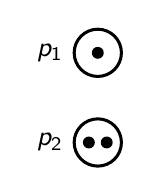
\begin{tikzpicture}
    \begin{scope}
        \node[place,tokens=1,label=left:$ p_1 $] (p1) {};

        \node[place,below=of p1, tokens=2,label=left:$ p_2 $] (p2) {};
    \end{scope}

\end{tikzpicture}
\end{document}